\documentclass[titlepage]{article}

\usepackage[czech]{babel}
\usepackage{graphicx}
\usepackage{tikz}
\usepackage{hyperref}
\usepackage{dirtree}
\usepackage{amsmath}
\usepackage{pdfpages}

\makeatletter
\tikzset{
    database/.style={
        path picture={
            \draw (0, 1.5*\database@segmentheight) circle [x radius=\database@radius,y radius=\database@aspectratio*\database@radius];
            \draw (-\database@radius, 0.5*\database@segmentheight) arc [start angle=180,end angle=360,x radius=\database@radius, y radius=\database@aspectratio*\database@radius];
            \draw (-\database@radius,-0.5*\database@segmentheight) arc [start angle=180,end angle=360,x radius=\database@radius, y radius=\database@aspectratio*\database@radius];
            \draw (-\database@radius,1.5*\database@segmentheight) -- ++(0,-3*\database@segmentheight) arc [start angle=180,end angle=360,x radius=\database@radius, y radius=\database@aspectratio*\database@radius] -- ++(0,3*\database@segmentheight);
        },
        minimum width=2*\database@radius + \pgflinewidth,
        minimum height=3*\database@segmentheight + 2*\database@aspectratio*\database@radius + \pgflinewidth,
    },
    database segment height/.store in=\database@segmentheight,
    database radius/.store in=\database@radius,
    database aspect ratio/.store in=\database@aspectratio,
    database segment height=0.1cm,
    database radius=0.25cm,
    database aspect ratio=0.35,
}
\makeatother



\title{Generátor úloh do aplikované kryptografie\\Dokumentace}
\author{Michal Homola,\\Dominik Chrenčík,\\Jiří Marák,\\Vojtěch Lukáš}

\begin{document}
\maketitle

\tableofcontents

\section*{Úvod}
\addcontentsline{toc}{section}{Úvod}
Předmětem této dokumentace je představit vyhotovení projektu s názvem \uv{Generátor kryptografických úloh}. První část bude věnována teoretickému popisu systému jako celku. V~druhé části bude názorně popsán průběh komunikace mezi serverem a klientem a ve třetí části bude ve stručnosti představeny zdrojové soubory. 

\section{Architektura}
Schéma systému lze vidět na obr.\,\ref{fig:sys}. Úlohy jsou uloženy v SQL databázi. K~této databázi má přístup pouze webový PHP~server. Ten slouží jako \uv{prostředník} mezi klientem a databází. Dále do úloh vkládá generované hodnoty (klíče apod.).
Klientská aplikace funguje jako přístupový bod a sehrává roli prezentační vrstvy. Pro jednoduchost je vyvinuta v jazyce Python, využívá pouze konzolové pro\-středí. 
\begin{figure}[h!]
    \centering
    

\begin{tikzpicture}
    \draw (-.5,0) node[database, label=below: SQL databáze, database radius = .5cm, database segment height = .25cm]{};
    \draw[densely dotted, thick] (0,0) -- (1.5,0);
    \draw (1.5, -.7) rectangle (2.5, .7);
    \draw (1.5, .35) -- (2.5, .35);
    \draw (1.5, 0) -- (2.5, 0);
    \draw (1.5, -.35) -- (2.5, -.35);
    \draw (2, -.7) node[below]{.NET server};

    \draw[dashed] (-2,-1.5) rectangle (3.5,1.5) coordinate (box_right);
    \draw (.75, 1.5) node[above]{Microsoft Azure};
    \draw[dashed] (box_right) ++(down: 1.5) -- ++(right: 2) coordinate (pc_left); 
    \draw (pc_left) rectangle ++(1, .75);
    \draw (pc_left) -- ++(-.25, -.25) -- ++(right: .75) coordinate (pc_text) -- ++(right: .25) -- ++(.25, .25);
    \draw (pc_text) node[below]{Python klient};

\end{tikzpicture}    
    \caption{Schéma systému}
    \label{fig:sys}
\end{figure}

\subsection{Konstrukce databáze}
V tabulce \ref{tab:struktura_databaze} lze vidět strukturu SQL databáze. 
Sloupec \textbf{ID} slouží jako primární klíč databáze, \textbf{Kód} úlohy pak slouží pro snazší rozlišení úloh. V~buňce \textbf{Zadání} se nachází textový popis úlohy. Zde stojí za povšimnutí, že všechny číselné hodnoty důležité k výpočtu jsou nahrazeny zástupnými znaky \uv{$\$n$}. 
Na místa těchto znaků bude logika v back-endu vkládat pseudonáhodně vygenerované hodnoty. Díky tomu bude možno jednu úlohu řešit vícekrát, po\-kaž\-dé s jinými parametry. 
Pole \textbf{Výsledek} je záměrně prázdné~--~správný výsledek zde vloží až server, který tuto hodnotu vypočítá podle vygenerovaných parametrů. 

Uživatel si bude moct vybrat jaký typ bude chtít řešit, back-end si tuto úlohu podle jejího kódu vytáhne z databáze, opatří ji vygenerovanými operandy a spolu se správným výsledkem a nápovědou ji zašle uživateli, jak lze vidět v diagramu na obr.\,\ref{fig:diagram}.


 \begin{table}[h]
    \centering
    \caption{Struktura SQL databáze}
    \label{tab:struktura_databaze}
    \vspace{.5em}
    \begin{tabular}[h]{| l | l | p{3.7cm} | l | l |}
        \hline
        \textbf{ID} & \textbf{Kód} & \textbf{Zadání} &  \textbf{Nápověda} & \textbf{Výsledek} \\
        \texttt{INT} & \texttt{VARCHAR(5)} & \texttt{TEXT} &  \texttt{TEXT} & \texttt{TEXT} \\
        \hline\hline
        1 & \texttt{PR} & Rozhodněte (ano/ne) zda je číslo $n=\$1$ prvočíslo  & \dots & \texttt{NULL} \\
        \hline
        2 & \texttt{RSAe} & Zašifrujte zprávu $m=\$1$, pomocí RSA kryptosystému. Prvočísla jsou $p=\$2;\ q=\$3$, a soukromý klíč je $e=\$4$  & \dots & \texttt{NULL} \\
        \hline
        \vdots & \vdots & \vdots & \vdots & \vdots \\
        \hline
    \end{tabular}
 \end{table}

 \subsection{Generátor hodnot}
Modul generace hodnot je pro tento projekt zcela klíčový. Byl implementován přímo v~rámci back-end serveru, taktéž v jazyce PHP. Pro každý typ úlohy byla vytvořena jedna funkce, která vygeneruje pseudonáhodné operandy a předá je jako svou návratovou hodnotu. 

Server pak podle kódu žádané úlohy zažádá o její prototyp SQL server a zavolá příslušnou funkci pro doplnění vygenerovaných hodnot. Takto upravenou úlohu zabalí jako JSON objekt a pošle uživateli. 

 \subsection{API}
Architektura back-endu je navržena podle doporučení REST API. Celé řešení je založeno na \cite{restapi}. Od začátku byl projekt vyvíjen přímo na serveru pro usnadnění přístupu. Všechny implementované dotazy jsou zmíněny v tabulce \ref{tab:api}.\footnote{\texttt{<url> = } \url{http://vut-fekt-mpckry-gr14.8u.cz/index.php}.}
\begin{table}[h!]
    \centering
    \caption{API funkce serveru} 
    \label{tab:api}
    \vspace{.5em}
    \begin{tabular}{|c|c|c|}
        \hline
        \textbf{URL} & \textbf{popis} & \textbf{použití} \\
        \hline \hline
        \texttt{/alltasks} & zašle všechny úlohy z DB & \texttt{<url>/alltasks} \\
        \hline
        \texttt{/task?code=<code>} &zašle úlohu s daným kódem & \texttt{<url>/task?code=pr} \\
        \hline
        \texttt{/randomtask} & zašle náhodnou úlohu & \texttt{<url>/randomtask}\\
        \hline
    \end{tabular}
\end{table}

Jako odpověď na tyto dotazy server zašle JSON objekt, který bude již obsahovat vygenerované hodnoty i výsledek. 

\section{Vývojový diagram}
Zjednodušený vývojový diagram je zobrazený na obr.\,\ref{fig:diagram}. Chronologicky program postupuje takto:
\begin{enumerate}
    \item Po spuštění Python klienta ihned zažádá o seznam všech úloh, které následně zobrazí uživateli.\footnote{Tyto úlohy \emph{nebudou obsahovat} vygenerované hodnoty, pouze zástupné znaky ($\$n$).} To vše pomocí HTTP GET po\-ža\-davku.
    \item Server jej příjme a na jeho popud zašle SQL query pro výběr \emph{všech} zá\-zna\-mů databázi. 
    \item Databáze zašle všechny své záznamy serveru.
    \item Server tuto odpověď zabalí do JSON objektu a zašle klientovi. 
    \item Uživateli se zobrazí všechny dostupné úlohy. Jednu z nich si vybere a zadá její kód.
    \item Klient na základě tohoto kódu opět vygeneruje  GET požadavek, který zašle serveru. 
    \item Server opět zasílá databázi (tentokrát již specifickou) SQL query. Žádá o jednu úlohu, jejíž kód se shoduje s kódem, který zadal uživatel. 
    \item Databáze zašle žádanou úlohu serveru. 
    \item Server pro tuto úlohu nyní vygeneruje operandy a správný výsledek. Operandy dosadí za tokeny \uv{$\$n$} v poli \texttt{description} a výsledek vloží do pole \texttt{result}. 
    \item Takto upravený záznam pak jako JSON objekt zašle klientovi.
    \item Klient zobrazí zadání úlohy (\texttt{description})\footnote{Popřípadě také nápovědu (\texttt{hint}) pokud si uživatel neví rady.} a čeká na uživatelem zadaný výsledek. Pokud uživatel zadal tentýž výsledek, který klientovi přišel ze serveru, je zvýšeno skóre a nabídnuto řešení další úlohy. V opačném případě se může uživatel pokusit o opětovné zadání výsledku, nebo sezení ukončit. 
\end{enumerate}
\begin{figure}[p]
    \centering
    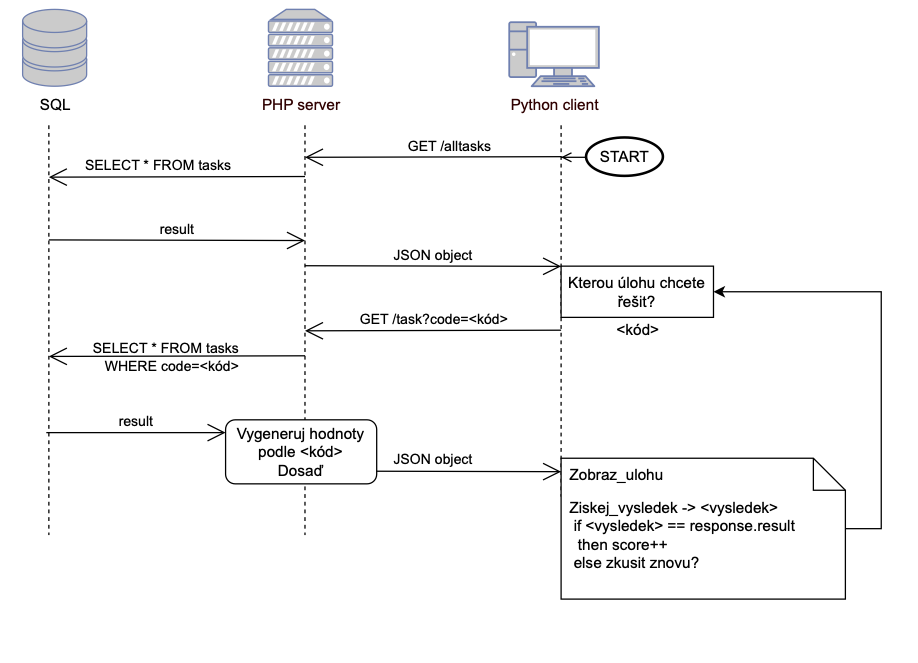
\includegraphics[width=.9\linewidth]{figures/diagram.png}
    \caption{Vývojový diagram systému}
    \label{fig:diagram}
\end{figure}

\section{Kód}
Adresářová struktura odevzdávaného projektu má tuto podobu:
\dirtree{%
    .1 /.
    .2 backend.
    .3 Controller.
    .4 Api.
    .5 BaseController.php.
    .5 TaskController.php.
    .4 Generator.php.
    .4 Populator.php.
    .3 Model.
    .4 Database.php.
    .4 TaskModel.php.
    .3 inc.
    .4 bootstrap.php.
    .4 config.php.
    .3 index.php.
    .2 frontend.
    .3 main.py.
    .3 clear\_console.py.
    .3 console\_colours.py.
    .3 print\_all\_tasks.py.
    .2 skupina14\_dokumentace.pdf.
}
Zdrojový kód je komentovaný, zde bude tedy pouze ve stručnosti popsána funkce jednotlivých modulů. 

\texttt{backend} obsahuje zdrojový kód PHP serveru. Klient se připojuje na koncový bod \texttt{index.php}~--~odtud jsou pak kaskádovitě volány další funkce, jejichž výsledkem je JSON objekt obsahující žádanou odpověď. Server \emph{neposkytuje} odpovědi jiného typu než JSON. Pro kontrolu není nutná instalace, server je veřejně přístupný na adrese \url{http://vut-fekt-mpckry-gr14.8u.cz/index.php/alltasks}.

\texttt{frontend} obsahuje zdrojový kód klienta. Hlavním souborem je \texttt{main.py}~--~ostatní soubory jsou pouze podpůrné. Skript se spouští bez argumentů. Testován byl ve verzi \texttt{Python 3.10.8}. Pro usnadnění spolupráce i kontroly byl tento skript také vyvěšen na tomto odkazu: \url{https://replit.com/@vlukas1/krygen-frontend?v=1}. Zde je i spustitelný. 

\section*{Závěr}
\addcontentsline{toc}{section}{Závěr}
Byl vyvinut stabilní systém pro generování a zasílání kryptografických úloh, který používá REST a JSON technologie. 

Díky oddělení funkčních prvků systému bylo možné jednoduše rozdělit práci mezi členy týmu a zrychlit tak vývoj. Systém je nyní modulární a lehce roz\-šiřitelný. Využitím JSON objektů je také velice univerzální. 



\begin{thebibliography}{9}
    \bibitem{restapi}
    SONI, Sajal. How to build a simple REST API in PHP. \emph{En\-va\-to Tuts+} [on\-li\-ne]. 27-5-2021 [cit. 2023-03-25]. Dostupné z: \url{https://code.tutsplus.com/tutorials/how-to-build-a-simple-rest-api-in-php--cms-37000}
\end{thebibliography}

    

\end{document}